\section{ОПРЕДЕЛЕНИЕ ПРЕДМЕТНОЙ ОБЛАСТИ И ТЕКУЩИХ РЕШЕНИЙ}

\subsection{Предметная область}

% \begin{definition}
%     \textbf{Прямоугольник} --- это четырехугольник с прямыми углами.
% \end{definition}

% \begin{lemma}
%     В прямоугольном треугольнике квадрат длины гипотенузы равен сумме квадратов длин катетов.
% \end{lemma}
% \proof
% Для начала, обозначим катеты прямоугольного треугольника $a$ и $b$, а гипотенузу $c$. Тогда по теореме Пифагора:

% \begin{equation}
%     a^2 + b^2 = c^2
% \end{equation}

% \begin{figure}[h]
%     \centering
%     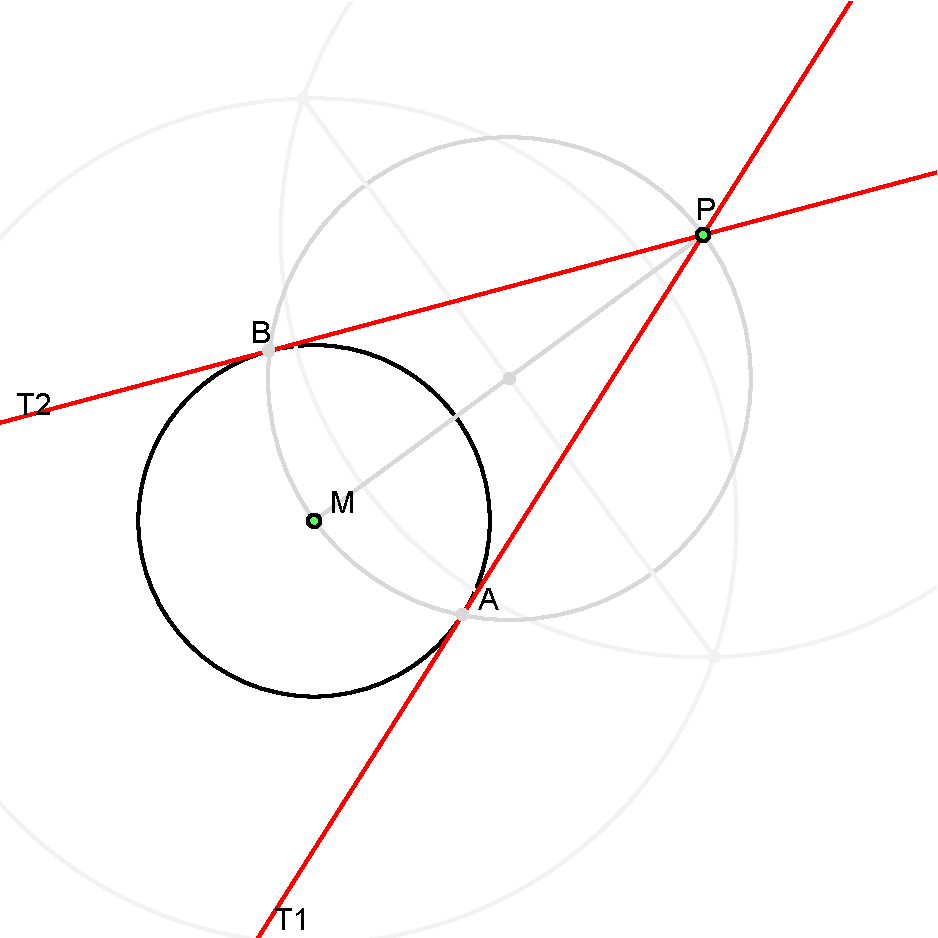
\includegraphics{math_geom_static_jsxgraph.pdf}
%     \caption{Название рисунка}
% \end{figure}

% \subsection{Второй подраздел}

% \begin{remark}
% Не все прямоугольники являются квадратами.
% \end{remark}

% \begin{example}
% Пример прямоугольника, который не является квадратом: прямоугольник со сторонами $3$ и $4$.
% \end{example}

% \begin{figure}[h]
%     \centering
%     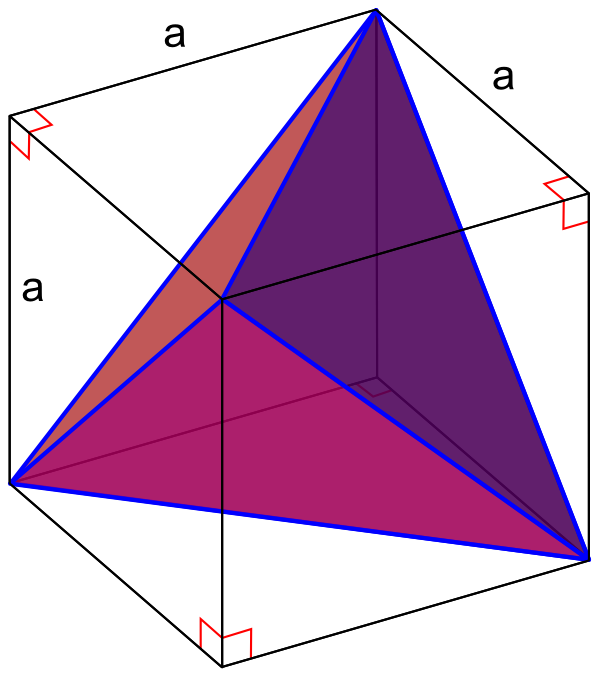
\includegraphics{regular_tetrahedron.png}
%     \caption{Название рисунка}
% \end{figure}

В научной литературе существует множество определений термина «большие данные». В рамках данной работы целесообразно выделить общие характеристики из всех предложенных определений. Распространённой ошибкой при определении понятия «большие данные» является попытка придать данным численную оценку объёма. Однако объём данных, классифицируемых как большие, не только постоянно увеличивается, но и зависит от возрастающих вычислительных мощностей систем, на которых эти данные обрабатываются и хранятся. Несмотря на необходимость дать численные оценки для данных, с которыми проводятся исследования, поскольку наша работа ограничена контекстом времени, это не противоречит основному свойству больших данных — их нельзя эффективно обработать или хранить на одном вычислительном узле. Следовательно, обработка таких объёмов данных требует использования горизонтально масштабируемых сервисов, как для обработки, так и для долговременного хранения данных [13].

Одной из распространённых платформ для хранения и анализа данных является Apache Hudi — транзакционная платформа данных, обеспечивающая соблюдение принципов ACID. В первом приближении Hudi можно охарактеризовать как формат хранения данных. Платформа способна использовать любое распределённое файловое хранилище, совместимое с S3, однако наибольшее распространение получила файловая система Hadoop Distributed File System (HDFS), являющаяся частью проекта Apache Hadoop. В данной работе выбор пал на HDFS, учитывая её популярность и совместимость с большинством сервисов для работы с большими данными.

В рамках данного исследования выбор конкретного файлового хранилища не является решающим, поскольку ключевым свойством всех подобных систем является высокая стоимость операций доступа к данным. Это обусловлено их распределённой архитектурой и необходимостью обмена данными по сети. Избежать данных затрат невозможно, учитывая, что объёмы хранимых данных могут достигать петабайтов, что делает вертикальное масштабирование чрезмерно дорогим или даже невозможным для таких систем. Кроме того, вертикальное масштабирование нецелесообразно, поскольку в распределённых файловых системах применяется репликация данных для обеспечения отказоустойчивости.

Apache Hudi поддерживает работу с историческими запросами: при обновлении набора данных создаётся новый снимок, в то время как предыдущий остаётся доступным. Каждый снимок соответствует определённому моменту времени на временной шкале, которая представляет собой журнал всех операций, выполненных над таблицей. Эта временная шкала позволяет отслеживать последовательность данных и обеспечивает доступ к информации для исторических запросов. На каждый момент времени приходится не более одного действия, создавая линейный порядок среди всех операций над таблицей. Каждое действие в журнале содержит информацию о времени (с точностью до миллисекунд), типе и состоянии операции. В данной работе рассматриваются только действия, связанные с модификацией данных. Состояние каждого действия может быть «запланировано», «в процессе» или «завершено». Таким образом, Hudi использует временную шкалу для оптимистичного управления параллельным доступом к данным.

В каждой таблице Hudi существует служебная директория, в которой находится вся метаинформация, необходимая для работы. Временная шкала находится в данной служебной директории, каждому состоянию действия соответствует один файл, название которого начинается с момента времени действия.

В рамках служебной директории располагается также таблица метаданных, которая является внутренней таблицей Hudi и остаётся скрытой от пользователя. Эта таблица интегрирована в пользовательскую таблицу, но недоступна для прямого доступа.

В Hudi различают два типа таблиц: 
\begin{enumerate}
    \item Copy-On-Write: данные хранятся в файлах с колоночно-ориентированным форматом. При операции записи генерируется новая версия файла данных, которая создаётся путём слияния существующего файла данных с новыми поступившими данными.
    \item Merge-On-Read: данные хранятся в файлах, сочетающих колоночно-ориентированный и строчно-ориентированный форматы. В процессе записи новые данные сначала сохраняются в дельта-файлах строчного формата, а затем сливаются с последней версией файла данных в процессе, известном как компактизация. 
\end{enumerate}
Компактизация может происходить как в синхронном, так и в асинхронном режиме.

Размер таблицы увеличивается с добавлением данных. Поскольку для размера файла данных существует определённый разумный предел, данные разделяются на файловые группы. При достижении заданного конфигурируемого предела размера файла данных формируется новая файловая группа. Записи с новыми ключами размещаются в новой файловой группе, в то время как обновления записей с уже известными ключами записываются в ту же файловую группу, где находится оригинальная запись. Независимо от типа таблицы, каждый файл данных ассоциирован с определённой файловой группой. Файловая группа обладает уникальным случайно генерируемым идентификатором, который фигурирует в начале названия каждого файла данных. Кроме того, каждый файл данных ассоциируется с моментом времени действия на временной шкале, который также указан в названии файла.

Файловые группы расположены в директориях файловой системы, причём путь к такой директории называется партицией. Путь для каждой файловой группы генерируется на основе пользовательски заданной схемы партиционирования. Схема партиционирования включает в себя список атрибутов таблицы, значения которых определяют путь расположения файловой группы. Эти значения атрибутов используются для оптимизации числа партиций, которые необходимо просканировать при выполнении запроса. Это означает, что если партиционирование выполнено по определённому атрибуту и запрос включает условие по этому атрибуту, процесс поиска местоположения файловой группы сводится к определению идентификатора этой группы.

Далее рассмотрим основные понятия, связанные с индексами. Индексы представляют собой структуры данных, возникшие из необходимости обеспечить быстрый поиск информации, хранящейся в базах данных. В отсутствие индексов поиск информации по всем записям, удовлетворяющим определённым критериям, требовал бы последовательного доступа к каждой записи для проверки её соответствия условиям. Для базы данных, содержащей N элементов, это потребовало бы времени порядка O(N), что для современных баз данных является неэффективным.

Индекс — это структура данных, которая позволяет ускорить процесс поиска за счёт использования дополнительного пространства и выполнения дополнительных операций записи для поддержания своей структуры. Существует множество типов индексов, предназначенных для работы с различными типами данных, такими как пространственные, временные, текстовые, многомерные и другие. Выбор подходящего индекса для конкретной задачи является ключевым аспектом процесса оптимизации, поскольку это может значительно влиять на временную сложность поиска, которая варьируется от O(logN) до O(1).

Учитывая изложенное, можно заключить, что задача определения расположения файла данных по заданному атрибуту с использованием индекса сводится к нахождению файловой группы, в которой расположена данная запись. В дальнейшем, для целей данной работы, термин «файловая группа» будет интерпретирован как «местоположение файла данных». При этом выбор конкретной версии файла данных в файловой группе зависит от типа запроса, включая исторические запросы. В рамках данной работы индекс будет отображать некоторые значения атрибутов на идентификатор файловой группы (расположение файла данных), в которой расположены соответствующие записи.